\documentclass{ximera}

\newcommand{\RR}{\mathbb R}
\renewcommand{\d}{\,d}
\newcommand{\dd}[2][]{\frac{d #1}{d #2}}
\renewcommand{\l}{\ell}
\newcommand{\ddx}{\frac{d}{dx}}
\newcommand{\dfn}{\textbf}
\newcommand{\eval}[1]{\bigg[ #1 \bigg]}


\outcome{Estimate partial derivatives from tables and graphs.}

\outcome{View the chain rule in terms of the gradient.}

\author{Bart Snapp}

\begin{document}
\begin{exercise}
  Let $F:\R^2\to\R$ be a differentiable function that is roughly
  described by the following table of values:
  \begin{image}
  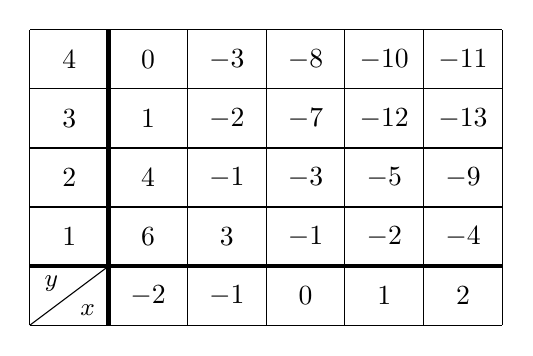
\begin{tikzpicture}[x=1cm,y=.75cm]
    \draw (0,0) grid [step=1] (6,5);
    
    \draw[ultra thick] (0,1)--(6,1);
    \draw[ultra thick] (1,0)--(1,5);
    
    \draw (0,0) -- (1,1);
    \node at (.4,.9) [below left,inner sep=1pt] {\small$y$};
    \node at (0.6,.1) [above right,inner sep=1pt] {\small$x$};
    
    %% y-values
    \node at (0.5,4.5) {$4$};
    \node at (0.5,3.5) {$3$};
    \node at (0.5,2.5) {$2$};
    \node at (0.5,1.5) {$1$};

    
    %% z-values
    %% top
    \node at (1.5,4.5) {$0$};
    \node at (2.5,4.5) {$-3$};
    \node at (3.5,4.5) {$-8$};
    \node at (4.5,4.5) {$-10$};
    \node at (5.5,4.5) {$-11$};
    
    %% 
    \node at (1.5,3.5) {$1$};
    \node at (2.5,3.5) {$-2$};
    \node at (3.5,3.5) {$-7$};
    \node at (4.5,3.5) {$-12$};
    \node at (5.5,3.5) {$-13$};
    
    %% 
    \node at (1.5,2.5) {$4$};
    \node at (2.5,2.5) {$-1$};
    \node at (3.5,2.5) {$-3$};
    \node at (4.5,2.5) {$-5$};
    \node at (5.5,2.5) {$-9$};
    
    %% 
    \node at (1.5,1.5) {$6$};
    \node at (2.5,1.5) {$3$};
    \node at (3.5,1.5) {$-1$};
    \node at (4.5,1.5) {$-2$};
    \node at (5.5,1.5) {$-4$};
    
    %% bottom row
    \node at (1.5,.5) {$-2$};
    \node at (2.5,.5) {$-1$};
    \node at (3.5,.5) {$0$};
    \node at (4.5,.5) {$1$};
    \node at (5.5,.5) {$2$};
  \end{tikzpicture}
  \end{image}
  Let $\vecl$ be the line running from the point $(2,1)$ to $(-2,5)$
  as $t$ runs from $0$ to $1$.  Estimate $\grad{F}(0,3)$ and use this
  to estimate $\dd{t}F(\vecl(t))$ at $t = 1/2$.
  \[
  \vecl(t) = \vector{\answer{2-4t},\answer{1+4t}}
  \]
  \[
  \grad F(0,3) \approx \vector{\answer{-5},\answer{-2.5}}
  \]
  \[
  \eval{\dd{t} F(\vecl(t))}_{t=1/2} \approx \answer{10}
  \]
\end{exercise}
\end{document}
